% Source: English Chapter 3, printed p. 89, PDF page 106.
\chapter{Nonlinear First-Order PDE}
\label{chap:nonlinear-first-order-pde}

\PDESource
  {Chapter 3; printed pp.~89--158; PDF pages~106--175}
  {中译本：第三章，书内第 61 页起；章首页为 PDF 第 79 页。}

\noindent\textit{Editorial study edition.}
This chapter reconstructs Evans's exposition and proofs in the source
order; it is not a verbatim transcription. Source theorem identifiers
are distinguished from our chapter-wide numbering. Expanded calculations,
Chinese mathematical annotations, figures, and exercise solutions are
editorial additions.

For $F=F(p,z,x)$ we study $F(Du,u,x)=0$, with $p$ denoting the gradient
variable and $z$ the function-value variable. The main route is
\[
 \begin{gathered}
 \text{envelopes and characteristic ODE}\\
 \longrightarrow\ \text{local smooth solutions}\\
 \longrightarrow\ \text{variational formulas and admissible weak solutions}.
 \end{gathered}
\]
\Needspace{45mm}
\PDEAnnotation{从局部光滑到全局弱解}{特征线在相空间中仍可光滑演化，但投影到物理空间后可能相交。单值光滑解因此失效；Hamilton--Jacobi 选择半凹分支，守恒律选择满足熵条件的跳跃。}
\paragraph{Conventions and prerequisites.}
Spatial gradients are column vectors. Time is a distinguished extra
coordinate for evolution equations. Hamiltonians and fluxes are real
valued; convexity and superlinearity are stated wherever used.
We use local ODE existence/uniqueness and smooth dependence, the implicit
and inverse function theorems, standard integration and weak derivative
calculus, Rademacher's theorem, and Gronwall's inequality as explicit
prerequisites. Supporting hyperplanes for finite convex functions are
invoked for the nonsmooth convex-duality statements.

\clearpage

% Evans second edition, section 3.1.
% English source: printed p. 90; PDF page 107 (1-based).
% Chinese section starts: checked against the chapter-opening list, PDF p. 79.
% Status: editorial study draft with detailed proofs and mathematical notes; no independent review.
\Needspace{65mm}
\section{Complete Integrals, Envelopes}
\label{sec:3-1}

\subsection{Complete integrals (Evans \S3.1.1)}
An $n$-parameter family $u(x;a)$ is a complete integral for
$F(Du,u,x)=0$ in $n$ independent variables if every member solves the
PDE and the $n\times(n+1)$ matrix
\[
 \bigl(D_a u,\ D^2_{ax}u\bigr)
\]
has rank $n$. The condition concerns variation of the whole first jet,
not only the gradient.
\Needspace{45mm}
\PDEAnnotation{完全积分不是所有解}{它是含足够独立参数的一族解，不能把“完全”理解成已经穷尽全部解。边界值通常是一整个函数，有限多个常数不能直接编码任意边界数据。}
If this family factored through $n-1$ parameters, $u(x;a)=v(x;\psi(a))$,
the chain rule would factor the displayed matrix through $D_a\psi$,
whose rank is at most $n-1$. Thus full rank rules out that redundancy.

\paragraph{Three useful families.}
For Clairaut's equation $x\cdot Du+f(Du)=u$,
\[
 u(x;a)=a\cdot x+f(a)
\]
solves the PDE and $D^2_{ax}u=I$, proving full rank.
For the eikonal equation $|Du|=1$, use $u=a\cdot x+b$ with $|a|=1$.
A local chart of the sphere has $n-1$ independent parameters and $b$
adds one; the independent tangential gradient variations and value
variation give rank $n$. This family is locally parametrized by an
open subset of $\R^n$, rather than treating the sphere as an open set.

For $u_t+H(D_xu)=0$ in $n+1$ independent variables,
\[
 u(x,t;a,b)=a\cdot x-tH(a)+b.
\]
There are $n+1$ parameters. The $a$ derivatives change $D_xu$ by the
standard basis, and the $b$ derivative changes the value by one
without changing the gradient. The corresponding jet matrix has
rank $n+1$, as required.

\subsection{Envelopes and singular integrals (Evans \S3.1.2, Theorem 1)}
\begin{theorem}\label{thm:3-envelope}
Let $U(x;a)$ be a smooth family of solutions and suppose
$D_aU(x;\alpha(x))=0$ with $\alpha$ continuously differentiable.
Then $v(x)=U(x;\alpha(x))$ is also a solution wherever this construction
is defined.
\end{theorem}
\begin{expandedproof}
For each coordinate, the full chain rule is
\[
 \partial_i v
 =\partial_{x_i}U(x;\alpha(x))
   +\sum_j\partial_{a_j}U(x;\alpha(x))\partial_i\alpha_j.
\]
The sum vanishes by the stationary-parameter condition. Thus $v$ and
the selected family member have the same value and the same spatial
gradient at $x$. Substitution into $F$ proves the PDE.
To obtain a smooth stationary parameter locally, one sufficient condition
is invertibility of $D^2_{aa}U$, by the implicit function theorem.
That condition is sufficient, not part of the abstract envelope identity.
\end{expandedproof}
\Needspace{45mm}
\PDEAnnotation{为何参数导数消失}{对 $U(x,\alpha(x))$ 求导时，不能忘掉参数链式项。正是 $D_aU=0$ 使它消失，包络与被选中的曲面才在该点相切。}

For $U(x,t;a)=a\cdot x-t|a|^2$, stationarity gives $a=x/(2t)$,
and the envelope is $v(x,t)=|x|^2/(4t)$ for $t>0$.
Indeed $v_t=-|x|^2/(4t^2)$ and $|D_xv|^2=|x|^2/(4t^2)$.
This example uses $H(p)=|p|^2$; later the common choice $H=|p|^2/2$
has a different factor of two.
\Needspace{45mm}
\PDEAnnotation{二次 Hamiltonian 的系数}{若 $H(p)=|p|^2$，其对偶为 $L(v)=|v|^2/4$；若 $H(p)=|p|^2/2$，则 $L(v)=|v|^2/2$。检查公式时，把 PDE、对偶与包络中的系数一起核对。}

For $U(x;a)=\pm\sqrt{1-|x-a|^2}$, the PDE is
$U^2(1+|DU|^2)=1$. Stationarity yields $a=x$ and the envelopes
$v=\pm1$. The derivative with respect to $a$ of the upper branch is
$(x-a)/\sqrt{1-|x-a|^2}$; changing the branch changes the sign.

One can restrict the parameters to $a=(a',h(a'))$ and then form an
envelope over $a'$. The stationary equations become
$U_{a_i}+U_{a_n}h_{a_i}=0$. The resulting general integral depends on
the arbitrary function $h$, whenever a smooth envelope exists.
It still need not describe every PDE solution: a factorized equation
$F_1(Du,u,x)F_2(Du,u,x)=0$ may have a branch belonging only to $F_2$.

\begin{center}
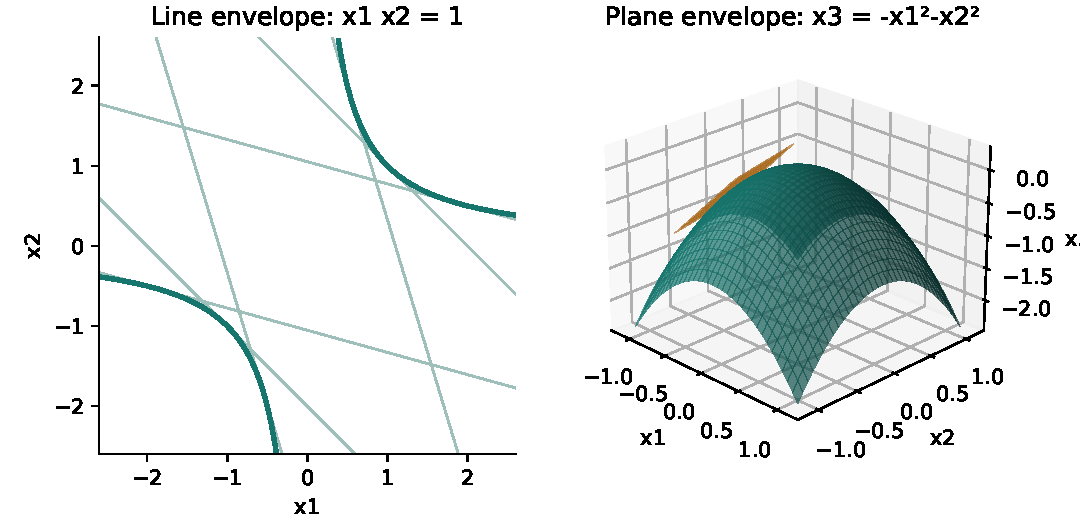
\includegraphics[width=\linewidth]{output/figures/ch03-envelopes.pdf}
\end{center}
\noindent\textit{Editorial figure for Problem 2.}
A hyperbola is tangent to a family of lines; a negative paraboloid
is tangent to the associated family of planes. Elimination and
parameter-domain restrictions are worked out in the exercise solution.

% Evans second edition, section 3.2.
% English source: printed p. 94; PDF page 111 (1-based).
% Chinese section starts: checked against the chapter-opening list, PDF p. 79.
% Status: editorial study draft with detailed proofs and mathematical notes; no independent review.
\Needspace{65mm}
\section{Characteristics}
\label{sec:3-2}

\subsection{Deriving the full characteristic system (Evans \S3.2.1)}
Suppose first that a $C^2$ solution exists. Along a curve $X(s)$ set
$Z(s)=u(X(s))$ and $P(s)=Du(X(s))$.
Then
\[
 \dot P_i=\sum_j u_{x_ix_j}(X)\dot X_j.
\]
Differentiate the PDE itself in $x_i$:
\[
 \sum_j F_{p_j}u_{x_jx_i}+F_z u_{x_i}+F_{x_i}=0.
\]
Choosing $\dot X_j=F_{p_j}$ makes the unknown Hessian sum match
the first expression. Hence
\[
 \boxed{\begin{aligned}
 \dot X&=F_p(P,Z,X),\\
 \dot P&=-F_x(P,Z,X)-F_z(P,Z,X)P,\\
 \dot Z&=P\cdot F_p(P,Z,X).
 \end{aligned}}
 \tag{CH}
\]
All partial derivatives of $F$ here hold its other arguments fixed.
The third equation is the chain rule for $u(X(s))$.
\Needspace{45mm}
\PDEAnnotation{选择路径是为了消去 Hessian}{任意路径的梯度变化含 $D^2u$，并不封闭。取速度 $F_p$ 后，恰好能用微分后的 PDE 替换这组二阶导数，得到只含 $X,P,Z$ 的 ODE。}

\paragraph{An invariant of the system.}
Even before knowing $P=Du$, solutions of (CH) satisfy
\[
 \frac d{ds}F(P,Z,X)
 =F_p\cdot(-F_x-F_zP)+F_z(P\cdot F_p)+F_x\cdot F_p=0.
\]
Initial data with $F(P(0),Z(0),X(0))=0$ therefore remain on the
PDE constraint surface. This invariant alone does not yet prove
that the transported vector $P$ is the gradient of a single-valued function.

\subsection{Reduced systems and explicit examples (Evans \S3.2.2)}
For $b(x)\cdot Du+c(x)u=f(x)$, only
\[
 \dot X=b(X),\qquad \dot Z=f(X)-c(X)Z
\]
are needed to compute values.
If $b=b(x,u)$, the value equation remains
$\dot Z=-c(X,Z)$ for $b(x,u)\cdot Du+c(x,u)=0$;
the path now depends on the unknown value.

\paragraph{Rotation.}
For $x_1u_{x_2}-x_2u_{x_1}=u$ in the first quadrant with
$u(r,0)=g(r)$,
\[
 X(s)=(r\cos s,r\sin s),\qquad Z(s)=e^s g(r).
\]
Thus
$u(x_1,x_2)=e^{\arctan(x_2/x_1)}g(\sqrt{x_1^2+x_2^2})$.
This is also immediate from $u_\theta=u$ in polar coordinates.

\paragraph{Value blow-up without crossing.}
For $u_{x_1}+u_{x_2}=u^2$, $u(x_1,0)=g(x_1)$,
\[
 X(s)=(r+s,s),\qquad Z(s)=\frac{g(r)}{1-sg(r)},
\]
so
\[
 u(x_1,x_2)=\frac{g(x_1-x_2)}
                      {1-x_2g(x_1-x_2)}
\]
on the connected region reached before a denominator vanishes.
If $g(r)>0$, the characteristic value blows up at $s=1/g(r)$.
Continuing the rational expression beyond its pole is not continuing
a finite classical solution through the blow-up time.
\Needspace{45mm}
\PDEAnnotation{两种失效机制}{半线性例子可在路径不相交时因 $Z$ 爆破失效；守恒律常见的是值仍有界、空间梯度先爆破。只检查特征线位置还不够。}

\paragraph{A fully nonlinear example.}
For $u_{x_1}u_{x_2}=u$, $u(0,r)=r^2$, compatibility gives
$P_2(0)=2r$ and $P_1(0)=r/2$ when $r\ne0$.
The system is $\dot P_i=P_i$, $\dot X_1=P_2$,
$\dot X_2=P_1$, $\dot Z=2P_1P_2$.
It integrates to
\[
 X_1=2r(e^s-1),\quad X_2=\tfrac r2(e^s+1),\quad Z=r^2e^{2s}.
\]
Since $4X_2-X_1=4r$ and $4X_2+X_1=4re^s$,
\[
 u(x_1,x_2)=\frac{(x_1+4x_2)^2}{16}.
\]
Direct differentiation verifies the PDE and boundary data everywhere.
The characteristic construction just given is locally invertible only
where $r\ne0$; the polynomial formula extends across the excluded locus.
An explicit extension does not mean the local existence theorem was
applicable at the characteristic boundary point $r=0$.

\subsection{Admissible and noncharacteristic data (Evans \S3.2.3)}
Flatten the initial hypersurface to $x_n=0$ and write its coordinates
as $y\in\R^{n-1}$. Prescribing $u(y,0)=g(y)$ fixes
\[
 Z(0)=g(y),\quad P_i(0)=g_{y_i}(y)\ (i<n),\quad
 F(P(0),g(y),(y,0))=0.
 \tag{IC}
\]
Only the normal derivative $P_n(0)$ remains to be found.
At an admissible root $p^0$, the sufficient condition
$F_{p_n}(p^0,g(y_0),(y_0,0))\ne0$
lets the implicit function theorem solve for a smooth branch $q_n(y)$.
Different roots may produce different local solutions; uniqueness is
relative to the chosen admissible branch.
\Needspace{45mm}
\PDEAnnotation{边界值没有给出完整梯度}{沿边界求导只能得到切向分量，法向分量要由 PDE 求出。代数方程可能无根或多根；非特征条件保证的是已选根附近的局部唯一分支。}

For a curved surface, choose a smooth extension of $g$ and write
$p=D_{\tan}g+\lambda\nu$, where $\nu$ is its unit normal.
Differentiating the scalar constraint in $\lambda$ gives
\[
 \frac d{d\lambda}F(D_{\tan}g+\lambda\nu,g,x)
       =F_p\cdot\nu.
\]
Thus the invariant geometric noncharacteristic condition is
$F_p\cdot\nu\ne0$: the characteristic velocity crosses the surface.
Changing the normal's orientation changes the sign, not this condition.

For example $u_{x_2}=0$ with data on $x_2=0$ is noncharacteristic.
The equation $u_{x_1}=0$ on the same boundary is characteristic:
nonconstant data in $x_1$ are incompatible, while constant data leave
the $x_2$ dependence undetermined. Failure of the hypothesis can mean
either nonexistence or nonuniqueness.


\PDEBodyDiagram{3.1}{Noncharacteristic data permit local reconstruction.}
{The projected characteristic direction is $F_p$. Transversality makes the initial-surface parameters together with the flow parameter independent local coordinates. A tangent direction makes this coordinate construction singular; it does not by itself prove that no solution can exist.}
{ch03-transverse}

\subsection{Reconstructing a local solution (Evans \S3.2.4, Theorem 2)}
\Needspace{45mm}
\PDEAnnotation{非特征条件是局部条件}{$F_p\cdot\nu\ne0$ 让特征穿过初始曲面，从而给出局部坐标。它不保证以后投影仍可逆；法向速度的正负另用于区分流入、流出方向。}
\begin{theorem}\label{thm:3-local}
For smooth $F,g$ and a chosen admissible noncharacteristic triple,
(CH) with data (IC) reconstructs a smooth local solution.
The construction is unique locally among smooth solutions sharing
that branch of boundary gradient.
\end{theorem}
\begin{expandedproof}[including the gradient compatibility step]
\paragraph{1. Solve the ODE with boundary parameters.}
Use the boundary-parameterized solution
\[
 (X,P,Z)(y,0)=((y,0),q(y),g(y)).
\]
Local ODE theory with smooth dependence supplies a common parameter neighborhood.
At $s=0$, the columns $X_{y_i}$ are $e_i$, $i<n$, and
$X_s=F_p$. Hence
\[
 \det D_{(y,s)}X(y_0,0)=F_{p_n}(p^0,z^0,x^0)\ne0.
\]
The inverse function theorem gives local coordinates
$(y,s)=(y(x),s(x))$. Define $u(x)=Z(y(x),s(x))$.

\paragraph{2. Preserve the algebraic PDE constraint.}
The invariant above and initial compatibility give
$F(P(y,s),Z(y,s),X(y,s))=0$.
We still have to prove $P(y,s)=Du(X(y,s))$.

\paragraph{3. Propagate the contact identities.}
The $s$ identity $Z_s=P\cdot X_s$ is in (CH).
For every boundary parameter set
$R_i=Z_{y_i}-P\cdot X_{y_i}$.
Initially $R_i=0$, by the tangential compatibility in (IC).
Differentiate:
\[
 \begin{split}
 (R_i)_s
 &=P_{y_i}\cdot X_s-P_s\cdot X_{y_i}\\
 &=F_p\cdot P_{y_i}+F_x\cdot X_{y_i}
                         +F_zP\cdot X_{y_i}.
 \end{split}
\]
Differentiating the preserved identity $F(P,Z,X)=0$ in $y_i$ yields
$F_p\cdot P_{y_i}+F_x\cdot X_{y_i}=-F_zZ_{y_i}$.
Therefore $(R_i)_s=-F_zR_i$ with zero initial value.
Uniqueness for this scalar linear ODE gives $R_i=0$.

\paragraph{4. Return to physical coordinates.}
Together the identities say $dZ=P\cdot dX$ for all parameter
differentials. Since $D_{(y,s)}X$ is invertible, every physical
differential occurs, so $Du=P$.
The preserved constraint now becomes $F(Du,u,x)=0$.
At $s=0$ we recover $u=g$. Any other smooth solution with the same
boundary gradient branch generates the same characteristic ODE data,
so ODE uniqueness and coordinate invertibility identify the solutions.
\end{expandedproof}
\Needspace{45mm}
\PDEAnnotation{不能提前把 $P$ 叫作梯度}{从 ODE 构造出来的 $P$ 起初只是向量场。必须证明 $dZ=P\cdot dX$，再利用坐标可逆性，才能认定 $P=Du$；否则只保留 $F(P,Z,X)=0$ 还没有解出 PDE。}

\subsection{Evolution equations and breakdown (Evans \S3.2.5)}
For $u_t+\mathbf f'(u)\cdot D_xu=0$ with initial data $g$,
\[
 X(a,t)=a+t\mathbf f'(g(a)),\qquad u(X(a,t),t)=g(a).
\]
Eliminating $a$ gives $u=g(x-t\mathbf f'(u))$ while the map is invertible.
Its Jacobian is $I+t\,\mathbf f''(g(a))\otimes Dg(a)$.
The rank-one determinant identity yields
\[
 \det D_aX=1+t\,Dg(a)\cdot\mathbf f''(g(a)).
\]
In one dimension,
\[
 u_x(X(a,t),t)=\frac{g'(a)}
                    {1+t f''(g(a))g'(a)}.
\]
If the denominator first vanishes with $g'(a)<0$ and $f''>0$,
gradients blow up although $u=g(a)$ remains finite.
For Burgers flux $f(u)=u^2/2$ and bounded $C^1$ data with
$m=\inf g'<0$, the first loss of a uniform positive Jacobian is at
$T_*=-1/m$. If the infimum is attained, that characteristic gives
an actual zero Jacobian at $T_*$.
\Needspace{45mm}
\PDEAnnotation{相空间不交不保证投影不交}{扩展状态 $(X,P,Z)$ 的 ODE 可保持唯一性，但只看 $X$ 时不同状态可落在同一位置。物理空间的逆映射失效，正是特征构造中光滑解失效的关键。}

For $u_t+H(D_xu,x)=0$, the full system becomes Hamilton's equations
and an action equation:
\[
 \dot X=H_p(P,X),\qquad
 \dot P=-H_x(P,X),\qquad
 \dot Z=P\cdot H_p-H.
\]
When $H=H(p)$, $P=Dg(a)$ stays constant and
\[
 X=a+tDH(Dg(a)),\qquad
 Z=g(a)+t[Dg(a)\cdot DH(Dg(a))-H(Dg(a))].
\]
This formula is local until the projection ceases to be invertible.
The next section gives a variational continuation with a selection rule.

% Evans second edition, section 3.3.
% English source: printed p. 110; PDF page 127 (1-based).
% Chinese section starts: checked against the chapter-opening list, PDF p. 79.
% Status: editorial study draft with detailed proofs and mathematical notes; no independent review.
\Needspace{65mm}
\section{Introduction to Hamilton--Jacobi Equations}
\label{sec:3-3}

\subsection{Variations and Hamilton's ODE (Evans \S3.3.1)}
For a path $X:[0,t]\to\R^n$ with fixed endpoints consider
\[
 \mathcal A[X]=\int_0^t L(\dot X(s),X(s))\,ds.
\]
Suppose a smooth minimizer exists. For every smooth variation $V$
vanishing at both endpoints, differentiate the action at $X+\varepsilon V$:
\[
 0=\int_0^t[L_v(\dot X,X)\cdot\dot V+L_x(\dot X,X)\cdot V]\,ds.
\]
Integration by parts, with the endpoint terms zero, gives
$\frac d{ds}L_v(\dot X,X)=L_x(\dot X,X)$ by the fundamental lemma
of the calculus of variations. These are the Euler--Lagrange equations.
They are necessary conditions; their derivation does not prove a
minimizer exists or that every stationary path minimizes.

Assume now the velocity--momentum relation $P=L_v(v,x)$ can be inverted,
and define
$H(P,x)=P\cdot v(P,x)-L(v(P,x),x)$.
In differentiating this identity the terms containing derivatives of
$v$ cancel because $P=L_v$. Thus $H_p=v$ and $H_x=-L_x$.
The Euler--Lagrange equations become
\[
 \dot X=H_p(P,X),\qquad \dot P=-H_x(P,X).
\]
For $L(v,x)=|v|^2/2-V(x)$ this gives $P=v$,
$H=|P|^2/2+V(x)$ and $\ddot X=-DV(X)$.
For an autonomous Hamiltonian,
$\frac d{ds}H=H_p\cdot(-H_x)+H_x\cdot H_p=0$.
\Needspace{45mm}
\PDEAnnotation{两个来源得到同一组 ODE}{变分法从作用量的驻值推出 Hamilton 方程；特征线法从 Hamilton--Jacobi PDE 推出同一方程。前者给出力学意义，后者解释它如何搬运函数与梯度。}

\subsection{Convex duality and Hopf--Lax (Evans \S3.3.2)}
\label{sec:3-hopflax}
A function $A$ is superlinear if $A(v)/|v|\to+\infty$ as $|v|\to\infty$.
For a finite convex function define
\[
 A^*(p)=\sup_v\{p\cdot v-A(v)\}.
\]
Superlinearity of $A$ makes the objective tend to $-\infty$,
so the maximum is attained and $A^*$ is finite.
It is convex as a supremum of affine functions.
For every $R>0$,
\[
 A^*(p)\geq R|p|-\max_{|v|=R}A(v);
\]
hence $A^*$ is also superlinear when $A$ is finite everywhere.

\begin{theorem}[Convex duality; source Theorem 3]
For finite convex superlinear $A$, $A^{**}=A$ and
\[
 A(v)+A^*(p)\geq p\cdot v.
\]
Equality holds precisely when $p$ is a supporting slope of $A$ at $v$.
For differentiable $A$, this means $p=DA(v)$.
\end{theorem}
\begin{expandedproof}
The inequality is the definition of the supremum.
A supporting slope satisfies
$A(w)\geq A(v)+p\cdot(w-v)$ for every $w$.
Rearranging shows the supremum defining $A^*(p)$ is attained at $v$,
giving equality. Conversely equality rearranges to that support inequality.
Always $A^{**}(v)\leq A(v)$. Choose a supporting slope at $v$;
then the equality just established gives the reverse inequality.
Existence of supporting hyperplanes for finite convex functions is
the invoked convex-analysis prerequisite.
For a differentiable convex function the tangent-plane inequality
provides this slope directly as $DA(v)$.
\end{expandedproof}
The supporting-plane argument for $A^{**}=A$ also holds for every
finite convex $A$ without superlinearity; in that case $A^*$ may take
the value $+\infty$. Subdifferentials of such extended-valued functions
are taken only at points where the function is finite.
\Needspace{45mm}
\PDEAnnotation{对偶变换中的极大值}{求 $v\cdot p-H(p)$ 的驻点只是候选；凸性让该目标关于 $p$ 凹，超线性增长使它在无穷远趋负无穷，才保证极大值确实取得。}

\PDEBodyDiagram{3.2}{Legendre duality is a supporting-line construction.}
{For $H(p)=p^2/2$ and $v=1$, maximizing $vp-H(p)$ finds the tangent point $p=1$. The tangent's intercept is $-L(1)=-1/2$. Convexity makes the whole graph lie above this line, which is exactly the Fenchel inequality.}
{ch03-legendre-support}

For the rest of this subsection assume $H$ is finite, convex, smooth
and superlinear on $\R^n$, set $L=H^*$, and let $g$ be globally
Lipschitz with constant $K$. Then $L$ is finite, convex and superlinear,
and $H=L^*$.

\Needspace{45mm}
\PDEAnnotation{超线性排除逃向远方的起点}{$g$ 的下降至多是线性的，而 $tL((x-y)/t)$ 在位移很大时增长更快。这不仅给出最小值存在，还把最优起点限制在 $|x-y|\leq Rt$ 内。}
\paragraph{Why a straight path gives the formula (source Theorem 4).}
Since $L$ no longer depends on position, Jensen's inequality gives
for any absolutely continuous path with $X(0)=y$, $X(t)=x$,
\[
 \int_0^tL(\dot X(s))\,ds
 \geq tL\left(\frac1t\int_0^t\dot X(s)\,ds\right)
 =tL((x-y)/t).
\]
The straight path $X(s)=y+s(x-y)/t$ attains equality.
Minimizing over its starting point gives
\[
 \boxed{u(x,t)=\min_{y\in\R^n}
             \{tL((x-y)/t)+g(y)\}.}
 \tag{HL}
\]
The minimum exists: with $v=(x-y)/t$, its objective is at least
$g(x)+t[L(v)-K|v|]$, coercive in $v$.
Comparing with $y=x$ also proves that every minimizer satisfies
$L(v)-K|v|\leq L(0)$, hence $|v|\leq R_K$ for a fixed finite $R_K$.
This is the first finite-range localization of the minimization.
\Needspace{45mm}
\PDEAnnotation{直线最优依赖哪些条件}{这里用到 $L$ 的凸性和无位置依赖。若 $L=L(v,x)$，不同路径经过不同势场，不能只用端点位移除以时间就替代整条作用量。}


\PDEMarginDiagram{3.M}{把路径在中途切开}
{中间点 $z$ 也要优化。两段代价相加后再取下确界，才得到动态规划恒等式。}
{ch03-path-split-margin}

\begin{lemma}[Dynamic programming; source Lemma 1]\label{lem:3-dpp}
For $0<s<t$,
\[
 u(x,t)=\min_z\{(t-s)L((x-z)/(t-s))+u(z,s)\}.
 \tag{DP}
\]
\end{lemma}
\begin{expandedproof}
For any $z$ and a minimizing starting point $y$ for $u(z,s)$,
convexity applied to
$(x-y)/t=[(t-s)/t](x-z)/(t-s)+(s/t)(z-y)/s$
gives
$u(x,t)\leq(t-s)L((x-z)/(t-s))+u(z,s)$.
This proves one inequality for the infimum over $z$.
Conversely take a minimizer $y$ in (HL) and choose
$z=y+(s/t)(x-y)$. Both subinterval velocities then equal $(x-y)/t$.
Use this same $y$ as a competitor for $u(z,s)$ to obtain the opposite
inequality. Coercivity ensures the intermediate minimum exists.
\end{expandedproof}

\begin{lemma}[Lipschitz bounds and initial values; source Lemma 2]
The function in (HL) is globally Lipschitz in $(x,t)$ for $t\geq0$,
when defined by $u(x,0)=g(x)$.
\end{lemma}
\begin{expandedproof}
If $y$ minimizes at $x$, use $y+h$ as competitor at $x+h$.
The velocity is unchanged, so $u(x+h,t)-u(x,t)\leq K|h|$.
Exchange $x,x+h$ for the reverse inequality.

For time zero, the competitor $y=x$ gives
$u(x,t)\leq g(x)+tL(0)$, while duality gives
\[
 u(x,t)\geq g(x)+t\inf_v[L(v)-K|v|]
 =g(x)-t\max_{|p|\leq K}H(p).
\]
Thus $|u(x,t)-g(x)|\leq Ct$, uniformly in $x$, with
\[
 C=\max\{|L(0)|,\max_{|p|\leq K}|H(p)|\}.
\]
Apply the same argument to (DP), using the spatial Lipschitz bound
for $u(\cdot,s)$, to get $|u(x,t)-u(x,s)|\leq C|t-s|$.
\end{expandedproof}


\PDEBodyDiagram{3.3}{Equal minimizing costs can produce a corner in the value.}
{With $H(p)=p^2/2$, $t=1$ and $g(y)=\max(-|y|,-2)$, the Hopf--Lax cost at $x=0$ has two minimizers $y=\pm1$. Their candidate endpoint slopes $(x-y)/t$ differ. Indeed near $x=0$ the value is $u(x,1)=-1/2-|x|$, so it is not differentiable there.}
{ch03-hopflax-tie}

\begin{theorem}[PDE at differentiability points; source Theorems 5--6]
The Hopf--Lax function satisfies $u_t+H(Du)=0$ at every point where
it is differentiable, hence almost everywhere by Rademacher's theorem.
\end{theorem}
\begin{expandedproof}
At a differentiability point $(x,t)$, (DP) with the competitor $x$
over a short forward time gives
$u(x+hv,t+h)\leq hL(v)+u(x,t)$ for every fixed $v$.
Divide by $h>0$ and pass to zero:
$u_t+v\cdot Du\leq L(v)$. Supremizing in $v$ yields
$u_t+H(Du)\leq0$.

For the other sign choose a minimizing $y$ in (HL) at $(x,t)$ and
put $v_*=(x-y)/t$.
At time $t-h$, $z=x-hv_*$ lies on the straight minimizing path.
Using $y$ as competitor there yields
$u(x,t)-u(z,t-h)\geq hL(v_*)$.
Differentiability gives $u_t+v_*\cdot Du\geq L(v_*)$.
Since $H(Du)\geq v_*\cdot Du-L(v_*)$, the reverse sign follows.
Neither argument differentiates a potentially nonsmooth minimizing
point $y(x,t)$.
\end{expandedproof}
\Needspace{45mm}
\PDEAnnotation{最小值不一定可微}{多个最优起点可能同时出现，不能直接对 $y(x,t)$ 求导。动态规划用固定竞争者给一侧不等式，再沿一条最优路径给另一侧，避开了这个问题。}

For $H(p)=|p|^2/2$, $L(v)=|v|^2/2$ and
$u(x,t)=\min_y\{|x-y|^2/(2t)+g(y)\}$.
At a smooth minimizing branch,
$(x-y)/t=Dg(y)$, so $x=y+tDg(y)$ and $Du=Dg(y)$,
recovering the local characteristic formulas.
When branches compete, the minimum remains meaningful even though
their smooth projection has broken down.

\subsection{Semiconcavity and uniqueness (Evans \S3.3.3)}
\label{sec:3-semiconcavity}
An a.e. PDE alone is insufficient for uniqueness.
For $H(p)=p^2$ and $g=0$ in one dimension, both $u=0$ and
\[
 v(x,t)=\min\{0,|x|-t\}
\]
are Lipschitz and satisfy $v_t+v_x^2=0$ off the three lines
$x=0,\pm t$. At the central upward corner,
$v(h,t)+v(-h,t)-2v(0,t)=2|h|$ for $|h|<t$.
This cannot be bounded by a constant times $h^2$.

\begin{definition}
A function $f$ is semiconcave with constant $C$ if
\[
 f(x+z)-2f(x)+f(x-z)\leq C|z|^2 .
\]
For continuous $f$ this is equivalent to concavity of
$f(x)-C|x|^2/2$, by the midpoint criterion and continuity.
For smooth $f$ it is equivalent to $D^2f\leq CI$.
\end{definition}
\Needspace{45mm}
\PDEAnnotation{半凹只限制向上弯曲}{允许向下尖角，禁止二阶差分过大的向上尖角。它不是要求 Hessian 的绝对值有界，也不是要求函数本身凹；先减去一个二次函数后才凹。}

\begin{theorem}[Source Lemmas 3--4]
If $g$ is semiconcave with constant $C$, the Hopf--Lax function has
the same spatial constant for all $t$.
If instead $D^2H\geq\theta I$, $\theta>0$, it satisfies
\[
 u(x+z,t)-2u(x,t)+u(x-z,t)\leq\frac{|z|^2}{\theta t},
\]
even for initial $g$ that is merely Lipschitz.
\end{theorem}
\begin{expandedproof}[including the dual estimate of Problem 15]
For the first assertion choose a minimizer $y$ at $(x,t)$.
Use $y+z$ and $y-z$ as competitors at $x+z$ and $x-z$.
All three velocities are equal, so their $L$ terms cancel.
The remaining second difference is that of $g$ at $y$.

For the second assertion, uniform convexity makes the maximizer $p(v)$
in $L(v)=\max_p(v\cdot p-H(p))$ unique, with $v=DH(p(v))$.
Strong monotonicity gives
\[
 \theta|p(v)-p(w)|^2
 \leq (v-w)\cdot(p(v)-p(w)),
\]
so $|p(v)-p(w)|\leq|v-w|/\theta$.
Comparing the optimizing expressions at $v$ and $v+h$ shows
$DL(v)=p(v)$; equivalently, apply the implicit function theorem
to $DH(p)=v$. Hence $DL$ is $1/\theta$-Lipschitz.
Integrating its increment along a segment gives
\[
 L(v+h)\leq L(v)+DL(v)\cdot h+\frac{|h|^2}{2\theta}.
\]
Add the estimates for $h$ and $-h$:
$L(v+h)+L(v-h)-2L(v)\leq|h|^2/\theta$.
Now use the same minimizing $y$ at all three target points.
The initial terms cancel and $h=z/t$ gives the claimed constant.

In particular, taking $v=(v_1+v_2)/2$, $h=(v_1-v_2)/2$ proves
\[
 \tfrac12L(v_1)+\tfrac12L(v_2)
 \leq L((v_1+v_2)/2)+\frac{|v_1-v_2|^2}{8\theta}.
\]
This is the dual inequality omitted from the source lemma's proof.
\end{expandedproof}

\begin{theorem}[Uniqueness in the source weak class; source Theorems 7--8]
Let $H$ be smooth, convex and superlinear. Among globally Lipschitz
functions with the same initial datum, satisfying the HJ equation a.e.
and the spatial semiconcavity bound
\[
 u(x+z,t)-2u(x,t)+u(x-z,t)
 \leq C(1+t^{-1})|z|^2,
\]
there is at most one solution.
The Hopf--Lax function belongs to this class if $g$ is semiconcave
or $H$ is uniformly convex.
\end{theorem}
\begin{expandedproof}[the source's regularized cone argument]
Let $w=u-\widetilde u$. Subtract the a.e. PDE and integrate $DH$
on the gradient segment:
\[
 w_t+b\cdot Dw=0,\qquad
 b=\int_0^1 DH(\lambda Du+(1-\lambda)D\widetilde u)\,d\lambda .
\]
Both gradients lie in a fixed ball, so $|b|\leq R$ for a finite $R$.

\paragraph{1. Smooth the coefficients, preserving a one-sided bound.}
Locally convolve $u,\widetilde u$ in space-time and define $b_\varepsilon$
by the same expression with their smoothed spatial gradients.
For $t>2\varepsilon$, semiconcavity implies
\[
 D^2u_\varepsilon,\ D^2\widetilde u_\varepsilon
      \leq C'(1+t^{-1})I .
\]
To check this, integrate their second-difference inequalities against
the nonnegative smoothing kernel, bound $1/s$ by $2/t$ on its time
support, then divide by the squared increment and let it tend to zero.
The gradients remain bounded and converge a.e. to the original ones.

Writing $A=D^2H\geq0$ and $B$ for the convex combination of smoothed
Hessians gives $B\leq C'(1+t^{-1})I$.
Thus $\operatorname{tr}(AB)\leq C'(1+t^{-1})\operatorname{tr}A$,
by conjugating with $A^{1/2}$ and taking traces.
Since $A$ is bounded on the gradient ball,
$\operatorname{div}b_\varepsilon\leq C''(1+t^{-1})$.
Also $|b_\varepsilon|\leq R$ and $b_\varepsilon\to b$ a.e.

\Needspace{45mm}
\PDEAnnotation{凸性把单边 Hessian 界传给速度}{两个半凹函数的 Hessian 只需有上界。因 $D^2H$ 半正定，迹运算仍给出 $\operatorname{div}b$ 的上界；若失去凸性，这一步的符号便没有保证。}
\paragraph{2. Integrate a nonnegative transform in a shrinking cone.}
Take a smooth nonnegative function $\phi$, and put $v=\phi(w)$.
Weak Lipschitz calculus gives $v_t+b\cdot Dv=0$ a.e.
On $B_{\rho(t)}(x_0)$, $\rho(t)=r+R(T-t)$ with $r>0$, set
$e(t)=\int v$. The moving-boundary term and $|b_\varepsilon|\leq R$
make its boundary flux nonpositive. For a.e. $t$ this yields
\[
 e'(t)\leq C''(1+t^{-1})e(t)
       +\int_{B_{\rho(t)}}(b_\varepsilon-b)\cdot Dv.
\]
These integrations hold for Lipschitz $v$ by approximation, or its
Sobolev integration formula on the smooth ball.
For each fixed $\delta>0$, the error tends to zero in $L^1(\delta,T)$
by dominated convergence on the compact cone.
Integrate against a nonnegative time test function and let
$\varepsilon\to0$, obtaining the same differential inequality without
the error on $[\delta,T]$.

\paragraph{3. Start Gronwall away from the singular time zero.}
Let $M$ be the sum of the time Lipschitz constants.
Since $w(\cdot,0)=0$, $|w(x,\delta)|\leq M\delta$.
Choose $\phi=\phi_\delta$ zero on $[-M\delta,M\delta]$ and strictly
positive outside. Then $e(\delta)=0$.
Gronwall on $[\delta,T]$ has a finite coefficient integral, and gives
$e(T)=0$. Hence $|w|\leq M\delta$ on $B_r(x_0)$ at time $T$,
using continuity to pass from a.e. points.
Let $\delta\downarrow0$. The ball and $T$ were arbitrary, so $w=0$.
Existence in the stated class follows from the two semiconcavity
estimates and the preceding Hopf--Lax theorem.
\end{expandedproof}
\Needspace{45mm}
\PDEAnnotation{不能从零时刻硬套 Gronwall}{$1/t$ 在零附近不可积。证明先用时间 Lipschitz 界把差值截掉，在正时刻 $\delta$ 得到零初始能量，再应用 Gronwall，最后令 $\delta\to0$。}

This is the semiconcavity-based weak formulation used in this chapter.
Viscosity solutions provide a broader comparison framework in Chapter 10;
the a.e. equation and the present selection condition must not be
silently interchanged.


% Evans second edition, section 3.4.
% English source: printed p. 130; PDF page 147 (1-based).
% Chinese section starts: checked against the chapter-opening list, PDF p. 79.
% Status: editorial study draft with detailed proofs and mathematical notes; no independent review.
\Needspace{65mm}
\section{Introduction to Conservation Laws}
\label{sec:3-4}

\subsection{Shocks and entropy (Evans \S3.4.1)}
We now work in one space dimension:
\[
 u_t+f(u)_x=0,\qquad u(x,0)=g(x).
\]
The conservative form must be retained after smoothness breaks down.
An integral solution is a locally bounded function satisfying
\[
 \int_0^\infty\!\!\int_{\R}[u\phi_t+f(u)\phi_x]\,dx\,dt
       +\int_{\R}g(x)\phi(x,0)\,dx=0
 \tag{CL}
\]
for every smooth compactly supported test function on $\R\times[0,\infty)$.
For smooth $u$, integration by parts proves equivalence with the PDE.
For discontinuous $u$, the expression $f'(u)u_x$ is not an ordinary
product of functions and cannot replace (CL) without additional theory.
\Needspace{45mm}
\PDEAnnotation{先守恒后求导}{光滑时 $f(u)_x=f'(u)u_x$；跳跃时 $u_x$ 含集中测度。守恒形式能直接对 $f(u)$ 作分布求导，避免给不连续函数与 Dirac 的乘积随意赋值。}

\begin{theorem}[Rankine--Hugoniot]\label{thm:3-rh}
Across a smooth shock curve $x=\gamma(t)$ with traces $u_l,u_r$,
an otherwise smooth integral solution must satisfy
\[
 \gamma'(t)(u_r-u_l)=f(u_r)-f(u_l).
 \tag{RH}
\]
For unequal states, the speed is the secant slope of $f$.
\end{theorem}
\begin{expandedproof}
Write locally $u=u_l+(u_r-u_l)\mathbf1_{\{x>\gamma(t)\}}$,
with the smooth extensions on each side understood.
The singular part of $u_t$ is $-\gamma'[u]\delta_{x=\gamma(t)}$;
that of $f(u)_x$ is $[f]\delta_{x=\gamma(t)}$.
Here $[u]=u_r-u_l$ and $[f]=f(u_r)-f(u_l)$.
The regular parts vanish by the PDE on each side.
The remaining distribution is zero precisely when (RH) holds.
Equivalently, integrate each smooth side of (CL) and add their
oppositely oriented interface fluxes.
\end{expandedproof}

For strictly convex $f$, an admissible shock has $u_l>u_r$.
Its speed satisfies
$f'(u_r)<\gamma'<f'(u_l)$, since secant slopes lie strictly between
endpoint tangent slopes.
Characteristics enter the shock from both sides.
An upward jump also satisfies (RH) with its secant speed, but would
send characteristics outward and is rejected by entropy.


\PDEBodyDiagram{3.4}{Shock speed is a secant slope.}
{For $f(u)=u^2/2$, the secant between $u_R=0.2$ and $u_L=1.4$ has slope $\sigma=0.8$. The tangent slopes satisfy $0.2<0.8<1.4$, so characteristics from both sides enter the shock. Reversing the spatial states keeps the secant slope but violates the compression direction.}
{ch03-flux-chord}

\paragraph{Why weak conservation alone is not unique.}
For Burgers flux $f(u)=u^2/2$ and data $g=0$ on $x<0$, $g=1$ on $x>0$,
both the upward step moving at speed $1/2$ and
\[
 u(x,t)=\begin{cases}
 0,&x\leq0,\\ x/t,&0<x<t,\\1,&x\geq t
 \end{cases}
\]
satisfy (CL). In the fan the PDE is
$-x/t^2+(x/t)(1/t)=0$, and both interfaces are continuous.
Each candidate attains the same initial data in local $L^1$.
Only the fan satisfies the one-sided bound derived below.
\Needspace{45mm}
\PDEAnnotation{跳跃条件不负责筛选方向}{Rankine--Hugoniot 只保证接口两侧通量守恒，上跳和下跳都可能满足。熵条件额外保留压缩型跳跃，排除向外散开的非物理解。}

\paragraph{Convex entropy pairs: an editorial explanation.}
For smooth convex $\eta$, define $q$ by $q'=\eta'f'$.
A smooth solution satisfies $\eta(u)_t+q(u)_x=0$.
For the viscous equation $u_t+f(u)_x=\varepsilon u_{xx}$,
\[
 \eta(u)_t+q(u)_x
 =\varepsilon\partial_{xx}\eta(u)
       -\varepsilon\eta''(u)|u_x|^2
 \leq\varepsilon\partial_{xx}\eta(u).
\]
If bounded viscous solutions converge strongly locally, their limit
therefore satisfies the distributional entropy inequality.
This is a conditional explanation of the selection rule, not a proof
of viscous existence or convergence.

For a downward shock $l=u_l>u_r=r$ with secant speed $s$, let
$C(v)=f(v)-f(r)-s(v-r)\leq0$ on $[r,l]$.
The singular entropy coefficient is
\[
 [q]-s[\eta]=-\int_r^l\eta'(v)C'(v)\,dv
            =\int_r^l\eta''(v)C(v)\,dv\leq0.
\]
Thus the convex entropy inequality selects the same direction.
For general nonsmooth solutions this chapter uses the source's
one-sided derivative condition as its explicit uniqueness class.

\subsection{The Lax--Oleinik construction (Evans \S3.4.2)}
\label{sec:3-laxoleinik}
Assume $f$ smooth and $f''\geq\theta>0$ on $\R$, and $g\in L^\infty$.
An additive constant in $f$ does not affect the PDE; take $f(0)=0$.
Let
\[
 P(x)=\int_0^xg(y)\,dy,\qquad
 L=f^*,\qquad G=(f')^{-1}=L'.
\]
The potential
\[
 W(x,t)=\min_y\{tL((x-y)/t)+P(y)\}
 \tag{LOP}
\]
is a Hopf--Lax solution of $W_t+f(W_x)=0$.
The candidate conservation-law solution is $u=W_x$ a.e.
\Needspace{45mm}
\PDEAnnotation{HJ 解是守恒律解的原函数}{$W_t+f(W_x)=0$ 对空间作分布求导，就得到 $u_t+f(u)_x=0$。给初始原函数 $P$ 加常数只会给 $W$ 加同一常数，不改变 $u$ 或最优起点。}
Since $f'$ is strictly increasing and onto, $G$ exists and is
$1/\theta$-Lipschitz. Differentiating the convex dual at its unique
maximizer gives $L'=G$ and $L''=1/f''(G)>0$.

\begin{theorem}[Source Theorem 1]\label{thm:3-lo}
For each $t>0$, minimizing starting points in (LOP) are ordered with $x$.
The minimizer is unique except at at most countably many $x$.
At differentiability points of $W$,
\[
 \boxed{u(x,t)=G((x-y(x,t))/t).}
 \tag{LO}
\]
\end{theorem}
\begin{expandedproof}
\paragraph{1. Ordering and countability.}
Put $c(x,y)=tL((x-y)/t)$.
Its mixed derivative is $c_{xy}=-L''((x-y)/t)/t<0$.
If $x_1<x_2$ and proposed minimizers had $y_1>y_2$,
integration of this mixed derivative on the rectangle gives
\[
 c(x_1,y_2)+c(x_2,y_1)<c(x_1,y_1)+c(x_2,y_2).
\]
Adding $P(y_1)+P(y_2)$ contradicts the sum of the two minimizing
inequalities. Hence every minimizer at $x_1$ is at most every minimizer
at $x_2$.
The minimum sets are nonempty compact sets by coercivity.
If a set has two distinct endpoints $y_-<y_+$, its interval
$(y_-,y_+)$ is disjoint from the corresponding intervals for other $x$.
Assigning a rational point to each nonempty interval proves there are
at most countably many such $x$.

\Needspace{45mm}
\PDEAnnotation{可数例外指固定的时间切片}{每个多重最优点对应一个互不相交的起点开区间，再各选一个有理数，才得到可数性。这不表示整个时空只存在可数个激波点，也不等于全局光滑。}
\paragraph{2. Differentiate the value without differentiating the optimizer.}
For a fixed minimizing $y$, use that same point as a competitor at
$x+h$. Then
$W(x+h,t)-W(x,t)\leq c(x+h,y)-c(x,y)$.
For positive and negative $h$, differentiability of $W$ gives
$W_x=L'((x-y)/t)=G((x-y)/t)$.
This works even if $P$ is not differentiable at the minimizing $y$.
Strict monotonicity of $G$ also forces uniqueness of $y$ at such a point.
\end{expandedproof}
\Needspace{45mm}
\PDEAnnotation{最优起点的跳跃产生激波}{$y(x,t)$ 保持单调，但可发生跳跃。跨过竞争分支时，$(x-y)/t$ 随之下降，因此 $u=G((x-y)/t)$ 出现向下跳跃；这把变分选择和熵方向联系起来。}

\begin{theorem}[Integral solution and initial trace; source Theorem 2]
The construction gives a bounded integral solution of (CL).
It satisfies $u(\cdot,t)\to g$ in $L^1_{\mathrm{loc}}$ as $t\downarrow0$.
\end{theorem}
\begin{expandedproof}
First $W$ is spatially Lipschitz with constant $\|g\|_\infty$, hence
$|u|\leq\|g\|_\infty$ a.e.
The a.e. HJ equation $W_t+f(W_x)=0$ is an equality of locally integrable
functions. Multiply it by $\phi_x$.
Integration by parts first in time and then in space gives
\[
 \iint W_t\phi_x
 =-\iint W\phi_{xt}-\int P\phi_x(\cdot,0)
 =\iint W_x\phi_t+\int g\phi(\cdot,0).
\]
All supports are compact and $W$ is Lipschitz; thus these are valid
weak integration identities. Substituting $u=W_x$ proves (CL).

To strengthen initial recovery, fix a Lebesgue point $x$ of $g$,
with value $g_0$. Then
$P(x+h)=P(x)+g_0h+o(|h|)$.
The coercive minimizer bound gives $|x-y|/t\leq R$ uniformly.
Writing $y=x-tv$, the minimizing objective becomes
\[
 P(x)+t[L(v)-g_0v]+o(t)
\]
uniformly for $|v|\leq R$.
The strictly convex function $L(v)-g_0v$ has unique minimizer
$v_*=f'(g_0)$. Compactness implies every minimizing velocity tends
to $v_*$: otherwise a convergent subsequence away from $v_*$ would
minimize the limiting strictly convex objective.
Formula (LO) therefore gives $u(x,t)\to G(v_*)=g_0$.
The uniform $L^\infty$ bound and dominated convergence on compact
intervals give the asserted local $L^1$ convergence.
\end{expandedproof}

\subsection{A one-sided estimate and uniqueness (Evans \S3.4.3)}
\label{sec:3-entropy}
For the Lax--Oleinik solution, choose a monotone minimizing
representative $y(x,t)$ (for example the largest minimizer).
For $z>0$,
$y(x+z,t)\geq y(x,t)$ and therefore
\[
 u(x+z,t)-u(x,t)\leq \frac{z}{\theta t}.
 \tag{OS}
\]
Indeed the corresponding velocity can increase by at most $z/t$;
$G$ is increasing and $1/\theta$-Lipschitz.
If the velocity decreases, the displayed upper bound is automatic.
Thus $u(x,t)-x/(\theta t)$ is nonincreasing at fixed $t$.
It has one-sided limits and only downward jumps, although its
decrease may be arbitrarily steep.
\Needspace{45mm}
\PDEAnnotation{单边界允许激波}{约束是 $u(x+z)-u(x)\leq Cz/t$，不是绝对值的 Lipschitz 界。向下跳跃完全允许，向上跳跃则被禁止；这正适合包含压缩激波的解空间。}

The source's entropy class consists of bounded integral solutions
with a representative satisfying
$u(x+z,t)-u(x,t)\leq C(1+t^{-1})z$ for $z>0$ a.e.
The term $1$ permits a more general bound than (OS).

\begin{theorem}[Source Theorem 3]
For smooth convex $f$, an entropy solution in this one-sided class
with a prescribed bounded initial datum is unique up to null sets.
Uniform convexity is used for the explicit Lax--Oleinik construction,
but plain convexity suffices for this uniqueness statement.
\end{theorem}
\begin{expandedproof}[dual transport, with two separate small-time scales]
Let $w=u-\widetilde u$ and
\[
 b(x,t)=\int_0^1f'(\lambda u+(1-\lambda)\widetilde u)\,d\lambda .
\]
Then $f(u)-f(\widetilde u)=bw$. Subtracting the two integral identities
with the same initial datum gives
\[
 \iint w(\phi_t+b\phi_x)=0
 \tag{DU}
\]
for tests compactly supported in $\R\times[0,\infty)$.
The common data cancel exactly; no pointwise initial derivative is assumed.

\paragraph{1. Regularize the velocity and control its upper derivative.}
Smooth bounded extensions of $u,\widetilde u$ in space-time by
nonnegative kernels and set
$b_\varepsilon=\int_0^1f'(\lambda u_\varepsilon+
(1-\lambda)\widetilde u_\varepsilon)\,d\lambda$.
The coefficients are uniformly bounded, say $|b_\varepsilon|\leq R$,
and converge a.e. to $b$.
For $t>2\varepsilon$, the one-sided bound, averaged against the kernel
and divided by $z$, gives
$(u_\varepsilon)_x,(\widetilde u_\varepsilon)_x
 \leq C'(1+t^{-1})$.
Because $f''\geq0$ and is bounded on the common bounded value range,
\[
 (b_\varepsilon)_x
 =\int_0^1 f''(\lambda u_\varepsilon+(1-\lambda)\widetilde u_\varepsilon)
       [\lambda(u_\varepsilon)_x+
                    (1-\lambda)(\widetilde u_\varepsilon)_x]\,d\lambda
 \leq C''(1+t^{-1}).
\]
Negative derivatives need no lower bound.

\paragraph{2. Solve a smooth backward test equation.}
Fix $\psi\in C_c^\infty(\R\times(0,T))$.
Let $v_\varepsilon$ solve
$(v_\varepsilon)_t+b_\varepsilon(v_\varepsilon)_x=\psi$ with
$v_\varepsilon(\cdot,T)=0$.
The characteristic formula is
\[
 v_\varepsilon(x,t)
 =-\int_t^T\psi(X_\varepsilon(s;x,t),s)\,ds,\qquad
 \dot X_\varepsilon=b_\varepsilon(X_\varepsilon,s).
\]
Bounded speed makes all its supports lie in a fixed spatial interval.
It vanishes near $T$, so it is an admissible smooth test in (DU).

For any fixed $\delta>0$, $\varepsilon<\delta/2$,
differentiate the flow in $x$:
\[
 \partial_xX_\varepsilon(s;x,t)
 =\exp\left(\int_t^s(b_\varepsilon)_x(X_\varepsilon(\tau),\tau)\,d\tau\right).
\]
The upper derivative bound for $t\geq\delta$ gives a uniform finite
bound on this positive factor.
Differentiating the test formula therefore yields
$|(v_\varepsilon)_x|\leq C_\delta$ for $\delta\leq t\leq T$.

\Needspace{45mm}
\PDEAnnotation{一维保序带来变差守恒}{光滑流关于初始位置严格递增，因此复合流只是重新排列同一条曲线上的取值次序，不增加总变差。这里不需要流的导数在零时刻附近有统一上界。}
\paragraph{3. A fixed early interval controls total variation.}
Choose a fixed $t_*>0$ so that $\psi=0$ for $0<t<2t_*$.
For $t\leq t_*$, $v_\varepsilon$ is transported unchanged along
characteristics to time $t_*$.
A one-dimensional smooth flow preserves order and is a diffeomorphism
of $\R$ (its speed is bounded). Hence composition with this flow
preserves total variation:
\[
 \int_{\R}|(v_\varepsilon)_x(x,t)|\,dx
 =\operatorname{Var}v_\varepsilon(\cdot,t)
 =\operatorname{Var}v_\varepsilon(\cdot,t_*)\leq D.
\]
The final bound follows from the derivative bound at the fixed $t_*$
and the fixed compact support. Crucially, $D$ is independent of both
$\varepsilon$ and a later splitting time $\delta<t_*$.

\paragraph{4. Pass the dual identity to the limit.}
Use $v_\varepsilon$ in (DU):
\[
 \iint w\psi=\iint w(b_\varepsilon-b)(v_\varepsilon)_x.
\]
Split at $t=\delta$, with $0<\delta<t_*$.
On $[\delta,T]$ the integrand tends to zero by dominated convergence,
using $C_\delta$ and common compact support.
On $(0,\delta)$, boundedness of $w,b_\varepsilon,b$ and the
total-variation estimate bound its absolute integral by $C D\delta$.
First let $\varepsilon\downarrow0$ for this fixed $\delta$,
then let $\delta\downarrow0$.
Thus $\iint w\psi=0$ for every interior test $\psi$, so $w=0$ a.e.
\end{expandedproof}
\Needspace{45mm}
\PDEAnnotation{两个小时间不能混用}{先固定源项消失的时段 $t_*$，用它得到统一的变差界；再另取 $\delta<t_*$ 切开误差。若让估计常数也随 $\delta$ 发散，就不能仅凭区间长度趋零断言误差消失。}


\subsection{Riemann's problem (Evans \S3.4.4, Theorem 4)}
For $g=u_l$ on $x<0$ and $g=u_r$ on $x>0$, the entropy solution for
a strictly convex flux is as follows.
If $u_l>u_r$, it is a shock with speed
$s=[f(u_l)-f(u_r)]/(u_l-u_r)$.
If $u_l<u_r$, it is the rarefaction
\[
 u(x,t)=\begin{cases}
 u_l,&x/t\leq f'(u_l),\\
 G(x/t),&f'(u_l)<x/t<f'(u_r),\\
 u_r,&x/t\geq f'(u_r).
 \end{cases}
 \tag{RF}
\]
Equal states give a constant solution.
\begin{expandedproof}
The shock satisfies the PDE off its interface, (RH) on it, and the
downward entropy direction.
In the fan, $u_t=-(x/t^2)G'(x/t)$ and
$f'(u)u_x=(x/t)G'(x/t)/t$, which cancel.
The fan joins continuously to both constant states and
$u_x=G'(x/t)/t\leq1/(\theta t)$.
Both candidates are integral solutions and approach their Riemann data
locally in $L^1$; the transition region has width $O(t)$.
The entropy uniqueness theorem just proved identifies them as the
selected solutions.
\end{expandedproof}
\begin{center}
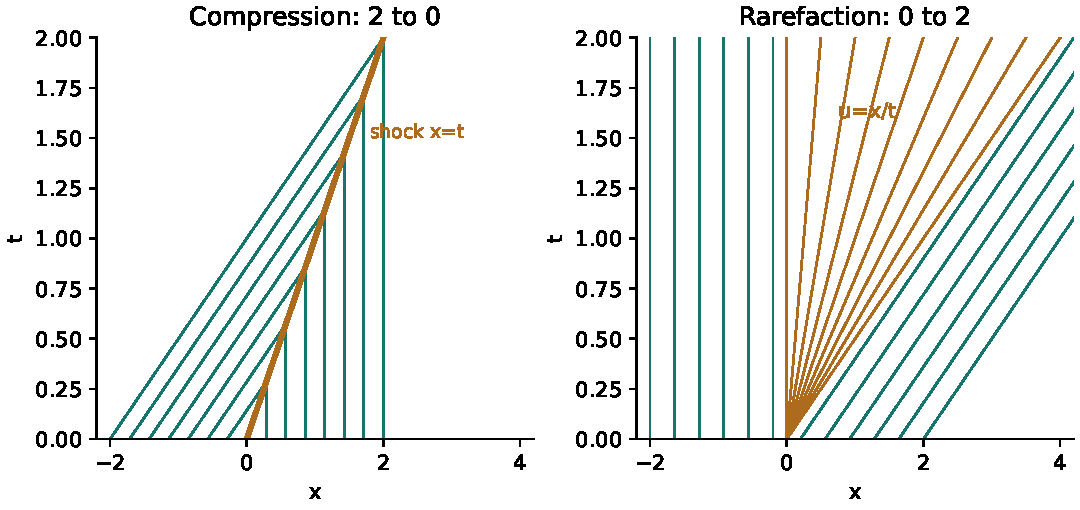
\includegraphics[width=\linewidth]{output/figures/ch03-riemann-characteristics.pdf}
\end{center}
\noindent\textit{Editorial figure.} For Burgers flow, a downward step
compresses characteristics into a shock; an upward step opens a
rarefaction fan. Both geometries use the same flux, but different data.

\subsection{Long-time decay and N-waves (Evans \S3.4.5)}
For this subsection assume $f(0)=0$, $f$ smooth, and
$0<\theta\leq f''\leq\Theta<\infty$.
These convenient sufficient hypotheses ensure uniform convexity of
both $f$ and $L=f^*$, as required in the source asymptotic arguments.
Write $\sigma=f'(0)$ and $d=f''(0)$.

\begin{theorem}[Supremum decay; source Theorem 5]
For bounded integrable initial data,
$\|u(\cdot,t)\|_\infty\leq C t^{-1/2}$.
\end{theorem}
\begin{expandedproof}
The primitive $P$ in (LOP) is bounded by $M=\|g\|_1$.
Duality gives $L(\sigma)=0$, $L'(\sigma)=0$.
Since $L''\geq1/\Theta$,
$L(v)\geq(v-\sigma)^2/(2\Theta)$.
Compare a minimizing $y$ with $y_0=x-\sigma t$:
\[
 \frac{|x-y-\sigma t|^2}{2\Theta t}-M
 \leq tL((x-y)/t)+P(y)\leq P(x-\sigma t)\leq M.
\]
Thus $|(x-y)/t-\sigma|\leq C/\sqrt t$.
As $G(\sigma)=0$ and $G$ is $1/\theta$-Lipschitz,
formula (LO) gives the claim.
\end{expandedproof}
\Needspace{45mm}
\PDEAnnotation{衰减的是高度，不一定是质量}{波的高度可按 $t^{-1/2}$ 降低，同时宽度按 $\sqrt t$ 增长。积分质量不一定趋零，所以长期形状应和一个展开的 N 波比较，而非只和零比较。}

Suppose additionally $\supp g\subset[-R,R]$.
Use the equivalent primitive $P(x)=\int_{-\infty}^xg$,
so $P_-=0$, $P_+=m=\int g$.
Let $P_*=\min P$,
\[
 p=-2P_*,\qquad q=2(m-P_*),\qquad p,q\geq0.
\]
The associated N-wave is
\[
 N(x,t)=\begin{cases}
 (x-\sigma t)/(dt),
   &-\sqrt{pdt}<x-\sigma t<\sqrt{qdt},\\
 0,&\text{otherwise}.
 \end{cases}
 \tag{NW}
\]
Its negative and positive signed areas are $-p/2$ and $q/2$,
so $\int N=(q-p)/2=m$.
\Needspace{45mm}
\PDEAnnotation{N 波参数由原函数最低点决定}{$p,q$ 不是初值正负质量各乘二。例如先取正脉冲再取等质量负脉冲，原函数始终非负且最终回零，此时 $p=q=0$，即使初值两种符号都有。}
\begin{theorem}[Source Theorem 6]
If $p,q>0$, then $\|u(\cdot,t)-N(\cdot,t)\|_1\leq C t^{-1/2}$.
\end{theorem}
\begin{expandedproof}[locating the edges before integrating the error]
Pass to the moving coordinate $\xi=x-\sigma t$ and put
$\ell(v)=L(\sigma+v)$. Then
$\ell(0)=\ell'(0)=0$ and $\ell''(0)=1/d$.
The minimizing velocity bound just proved is $|(\xi-y)/t|\leq C/\sqrt t$.
Taylor expansion on this fixed small-velocity range gives
\[
 t\ell((\xi-y)/t)=\frac{(\xi-y)^2}{2dt}+O(t^{-1/2}),
\]
\[
 u(x,t)=\frac{\xi-y(x,t)}{dt}+O(t^{-1}).
 \tag{NT}
\]
The constants are uniform for minimizers; the same Taylor bound holds
for the bounded starting-point competitors used below when $|\xi|=O(\sqrt t)$.

Choose $\varepsilon=A/\sqrt t$ with a fixed sufficiently large $A$.
We work for large $t$, so $\varepsilon<1$.

\paragraph{1. Exterior edges: the solution is zero beyond them.}
If $\xi<-R-\sqrt{pd(1+\varepsilon)t}$, the competitor $y=\xi$ has
objective $P_-=0$.
A minimizing $y\geq-R$ would, by (NT), have objective at least
\[
 \frac{pd(1+\varepsilon)t}{2dt}+P_*+O(t^{-1/2})
 =\frac{pA}{2\sqrt t}+O(t^{-1/2})>0.
\]
This contradicts the competitor when $A$ is large enough.
Thus $y<-R$, where $P=0$, and the strictly positive cost $\ell$
is minimized only by $y=\xi$. Hence $u=G(\sigma)=0$.
The right-tail argument is the same with the baseline $P_+=m$ and $q$.
Therefore $u=0$ outside
\[
 -R-\sqrt{pd(1+\varepsilon)t}
 \leq \xi\leq
 R+\sqrt{qd(1+\varepsilon)t}.
 \tag{OUT}
\]

\paragraph{2. Interior edges: the minimizing point stays in the initial support.}
At $\xi_l=R-\sqrt{pd(1-\varepsilon)t}$, any $y<-R$ has objective
at least $P_-=0$. Choose a point $z\in[-R,R]$ with $P(z)=P_*$.
Since $|\xi_l-z|\leq\sqrt{pd(1-\varepsilon)t}$ for large $t$,
its objective is at most
\[
 \frac{p(1-\varepsilon)}2+P_*+O(t^{-1/2})
 =-\frac{pA}{2\sqrt t}+O(t^{-1/2})<0.
\]
Thus every minimizer at $\xi_l$ is at least $-R$.
Similarly at $\xi_r=-R+\sqrt{qd(1-\varepsilon)t}$ it is at most $R$.
Monotonicity of minimizers then gives $|y(x,t)|\leq R$
throughout $\xi_l<\xi<\xi_r$.
There (NT) implies
$|u(x,t)-\xi/(dt)|\leq C/t$.

\paragraph{3. Integrate over the middle and the transition strips.}
The middle interval has length $O(\sqrt t)$ and lies inside the ideal
N-wave interval, so its $L^1$ error is $O(t^{-1/2})$.
Each strip between the interior, ideal, and exterior edges has bounded
length, since
$\sqrt{(1\pm A/\sqrt t)t}-\sqrt t=O(1)$.
Both $|u|$ and $|N|$ are $O(t^{-1/2})$, giving the same error there.
Outside (OUT) both are zero. This proves the bound for large times.

For a bounded time interval the minimizing-velocity bound from (HL)
gives finite propagation of the compact support and $|u|\leq\|g\|_\infty$.
Thus $\|u\|_1$ is uniformly bounded on that interval; $\|N\|_1=(p+q)/2$.
Enlarge $C$ to cover all remaining $t>0$.
\end{expandedproof}
\Needspace{45mm}
\PDEAnnotation{边缘位置也要估计}{只有波内 $O(1/t)$ 点态误差还不够做全空间积分。还要把两侧支集误差压进宽度 $O(1)$ 的条带，再乘以高度 $O(t^{-1/2})$，才能得到总误差。}

For Burgers flow with initial data $\mathbf1_{(0,1)}$, the fan is $u=x/t$.
Until $t=2$ it meets a height-one plateau ending at shock $x=1+t/2$.
After $t=2$ the shock is $x=\sqrt{2t}$ and
$u=x/t$ on $0<x<\sqrt{2t}$, zero elsewhere.
This follows from the fan--shock matching equation
$\gamma'=\gamma/(2t)$ and $\gamma(2)=2$.
It has height $O(t^{-1/2})$ and constant mass one.
Here $p=0$, $q=2$; the explicit example illustrates decay, while
the general $L^1$ theorem above was stated with $p,q>0$.


% Evans second edition, section 3.5.
% English source: printed p. 154; PDF page 171 (1-based).
% Chinese section starts: checked against the chapter-opening list, PDF p. 79.
% Status: editorial study draft with detailed proofs and mathematical notes; no independent review.
\Needspace{65mm}
\section{Problems}
\label{sec:3-5}

\noindent\textit{Source: Evans \S3.5, Problems 1--20, printed pp.~154--158
(PDF pp.~171--175).} Statements below are concisely restated.
All solutions are editorial, with smoothness assumed where required;
extensions beyond the smooth class are identified explicitly.

\subsection{Problems 1--8: envelopes and characteristics}
\Needspace{30mm}
\paragraph{1. A complete Hamilton--Jacobi integral.}
\begin{proof}[Solution]
For $U=a\cdot x-tH(a)+b$, $D_xU=a$ and $U_t=-H(a)$, proving the PDE.
There are $n+1$ parameters for $n+1$ independent variables.
The derivatives with respect to $a_i$ independently vary $D_xU$;
the derivative with respect to $b$ changes the value by one without
changing any gradient component.
These $n+1$ jet variations are linearly independent, proving completeness.
\end{proof}

\Needspace{30mm}
\paragraph{2. Envelopes of lines and planes.}
\begin{proof}[Solution]
For $G=x_1+a^2x_2-2a$, the stationary condition is $G_a=2ax_2-2=0$.
Thus $a\ne0$, $x_2=1/a$, and $G=0$ then gives $x_1=a$.
The envelope is $x_1x_2=1$, with both branches represented.
The line with $a=0$ has no finite stationary contact.
For $G=2a_1x_1+2a_2x_2-x_3+a_1^2+a_2^2$,
stationarity yields $a_i=-x_i$ and elimination gives
$x_3=-x_1^2-x_2^2$.
The derivatives of this paraboloid equal the slopes $2a_i$ of the
selected plane, directly verifying tangency. The figure in \S3.1
shows both constructions.
\end{proof}

\Needspace{30mm}
\paragraph{3. Eliminate parameters to obtain a PDE.}
\begin{proof}[Solution]
(a) For $\sum_i a_ix_i^2+u^3=0$, implicit differentiation gives
$2a_ix_i+3u^2u_{x_i}=0$.
Multiply by $x_i$, sum, and eliminate $\sum_i a_ix_i^2=-u^3$:
\[
 u^2(3x\cdot Du-2u)=0.
\]
On a nonzero branch this is $3x\cdot Du=2u$.
For a $C^1$ graph it extends to the zero set by continuity from
nonzero points, while on the interior of $\{u=0\}$ the gradient is zero.
This avoids division by a possibly zero coordinate $x_i$.

(b) A unit sphere centered at $(a,0)$ has
$|x-a|^2+u^2=1$. Differentiation yields $x-a=-uDu$.
Substitution eliminates $a$ and gives $u^2(1+|Du|^2)=1$,
on regions where the sphere is a differentiable graph.
\end{proof}
\Needspace{45mm}
\PDEAnnotation{参数消元要记录分支}{除以 $u$、$x_i$ 或某个行列式前，先说明它不为零。得到的简化 PDE 可能丢掉零解或特殊分支；保留未约去的形式有助于检查。}

\Needspace{30mm}
\paragraph{4. Forced transport.}
\begin{proof}[Solution]
For $u_t+b\cdot Du=f(x,t)$, use time as the characteristic parameter:
$\dot X=b$, $\dot Z=f(X,s)$.
Starting from the target, $X(s)=x-(t-s)b$.
Therefore
\[
 u(x,t)=g(x-tb)+\int_0^tf(x-(t-s)b,s)\,ds.
\]
This is the same formula as in Chapter 2.
In the full characteristic system the spatial gradient satisfies
$\dot P=D_xf$ and the time-gradient component satisfies $\dot Q=f_t$.
\end{proof}

\Needspace{30mm}
\paragraph{5. Three characteristic calculations.}
\begin{proof}[Solution]
(a) For $x_1u_{x_1}+x_2u_{x_2}=2u$, start at $(a,1)$.
Then $X=(ae^s,e^s)$, $Z=e^{2s}g(a)$.
For $x_2>0$, $s=\log x_2$ and $a=x_1/x_2$, so
$u=x_2^2g(x_1/x_2)$.

(b) For $x_1u_{x_1}+2x_2u_{x_2}+u_{x_3}=3u$,
start at $(a,b,0)$.
Then $X=(ae^s,be^{2s},s)$, $Z=e^{3s}g(a,b)$, giving
$u(x)=e^{3x_3}g(x_1e^{-x_3},x_2e^{-2x_3})$.

(c) For $uu_{x_1}+u_{x_2}=1$, start at $(a,a)$ with $Z(0)=a/2$.
The equations integrate to
\[
 X_2=a+s,\qquad Z=a/2+s,\qquad X_1=a+(a/2)s+s^2/2.
\]
Eliminate $s=X_2-a$:
$X_1=a(1-X_2/2)+X_2^2/2$.
Thus
\[
 a=\frac{2x_1-x_2^2}{2-x_2},\qquad u(x_1,x_2)=x_2-a/2
\]
locally near boundary points $(a,a)$ with $a\ne2$.
The parameter Jacobian is $1-x_2/2$.
At $(2,2)$ the boundary conditions themselves are incompatible:
Tangential differentiation gives $u_{x_1}+u_{x_2}=1/2$,
whereas the PDE and $u=1$ give the same left side equal to one.
There is no $C^1$ solution through that boundary point.
\end{proof}

\Needspace{30mm}
\paragraph{6. Flow Jacobians and a continuity equation.}
\begin{proof}[Solution]
Let $X(s;x,t)$ solve $\dot X=b(X)$ with $X(t;x,t)=x$.
On any interval where the smooth flow exists, its derivative matrix
$M=D_xX$ satisfies $M_s=Db(X)M$ and $M(t)=I$.
Jacobi's determinant formula gives
\[
 J_s=\operatorname{tr}(M^{-1}Db(X)M)J=(\operatorname{div}b)(X)J,
 \quad J(t)=1.
\]
In particular $J>0$ and is the exponential of the divergence integral.
For the forward map $Y(t;a)$, the desired density satisfies
\[
 \frac d{dt}\big[u(Y(t;a),t)\det D_aY(t;a)\big]=0.
\]
Set the product equal to $g(a)$; differentiating proves
$u_t+b\cdot Du+u\operatorname{div}b=0$.
Inverting the flow then gives
$u(x,t)=g(X(0;x,t))J(0;x,t)$.
A smooth vector field need not have a global complete flow; the formula
is asserted on its actual existence interval unless completeness is assumed.
\end{proof}

\Needspace{30mm}
\Needspace{45mm}
\PDEAnnotation{密度与被搬运的数值不同}{连续性方程保持的是 $u(Y,t)\det D_aY$，因为体积也在变化；纯传输保持 $u(Y,t)$。当速度无散时 Jacobian 为一，两者才在这一点上重合。}
\paragraph{7. A curved noncharacteristic surface.}
\begin{proof}[Solution]
The tangential boundary gradient is fixed. Write admissible gradients
as $D_{\tan}g+\lambda\nu$.
The derivative of their scalar PDE constraint in $\lambda$ is
$F_p\cdot\nu$. Nonvanishing permits local implicit solution for the
normal component. Equivalently, the characteristic column $F_p$ and
the boundary tangent columns form a basis exactly when this scalar
product is nonzero.
\end{proof}

\Needspace{30mm}
\paragraph{8. Verify the implicit conservation formula.}
\begin{proof}[Solution]
Let $a=x-t\mathbf f'(u)$ and $u=g(a)$.
With $D=1+tDg(a)\cdot\mathbf f''(u)\ne0$, differentiate:
\[
 Du=\frac{Dg(a)}D,\qquad
 u_t=-\frac{Dg(a)\cdot\mathbf f'(u)}D.
\]
Hence $u_t+\mathbf f'(u)\cdot Du=0$.
The nonzero denominator is exactly the rank-one determinant from the
characteristic projection. Its loss is not repaired by the implicit
formula itself.
\end{proof}

\subsection{Problems 9--16: variations and convex duality}
\Needspace{30mm}
\paragraph{9. A free initial endpoint.}
\begin{proof}[Solution]
Variations have $V(t)=0$ but arbitrary $V(0)$.
After integration by parts the first variation is
\[
 \int_0^t\left[L_x-\frac d{ds}L_v\right]\cdot V\,ds
                  -L_v(\dot X(0),X(0))\cdot V(0).
\]
First choose $V(0)=0$ to obtain the Euler--Lagrange equation.
Then arbitrary $V(0)$ gives $L_v(\dot X(0),X(0))=0$.
Adding the initial cost $g(X(0))$ adds
$Dg(X(0))\cdot V(0)$, so the new boundary condition is
$L_v(\dot X(0),X(0))=Dg(X(0))$.
\end{proof}
\Needspace{45mm}
\PDEAnnotation{初始代价决定初始动量}{自由起点不代表可以忽略端点项。变分边界项的负号与 $g(X(0))$ 的变化抵消后，得到 $P(0)=Dg(X(0))$，恰好接上 HJ 特征初值。}

\Needspace{30mm}
\paragraph{10. Two Legendre transforms.}
\begin{proof}[Solution]
(a) For $H(p)=|p|^r/r$, $1<r<\infty$, the maximizer of $v\cdot p-H(p)$
is parallel to $v$, with $|p|^{r-1}=|v|$.
Writing $1/r+1/s=1$ gives $L(v)=|v|^s/s$, also valid at $v=0$.
(b) For $H(p)=\tfrac12p^TAp+b\cdot p$, $A$ symmetric positive definite,
stationarity gives $p=A^{-1}(v-b)$.
Substitution gives $L(v)=\tfrac12(v-b)^TA^{-1}(v-b)$.
Positive definiteness makes this stationary point the unique global maximum
of the concave objective.
\end{proof}

\Needspace{30mm}
\paragraph{11. Subdifferential reciprocity.}
\begin{proof}[Solution]
The condition $v\in\partial H(p)$ is
$H(q)\geq H(p)+v\cdot(q-p)$ for every $q$.
It is equivalent to $p$ maximizing $v\cdot q-H(q)$,
hence to $H(p)+L(v)=p\cdot v$.
Using $H=L^*$, the same argument with the roles exchanged is equivalent
to $p\in\partial L(v)$.
For nonsmooth finite convex functions, this uses the supporting-hyperplane
version of the duality established above, rather than an unjustified gradient.
\end{proof}

\Needspace{30mm}
\paragraph{12. A finite-dimensional dual minimum.}
For smooth convex superlinear $L_i$ and $H_i=L_i^*$, prove
\[
 \min_v[L_1(v)+L_2(v)]=\max_p[-H_1(p)-H_2(-p)].
\]
\begin{proof}[Solution]
For any $v,p$, Fenchel's inequalities give
$L_1(v)+L_2(v)\geq-H_1(p)-H_2(-p)$.
The convex superlinear sum has a minimizing $v_*$.
Smoothness gives $DL_1(v_*)+DL_2(v_*)=0$.
Choose $p_*=DL_1(v_*)=-DL_2(v_*)$.
Both Fenchel inequalities are equalities for this pair.
Thus the minimum equals the stated dual maximum, which is attained at $p_*$.
\end{proof}

\Needspace{30mm}
\paragraph{13. A sharper finite-speed radius.}
\begin{proof}[Solution]
Assume here the source's smooth initial datum, with bounded gradient.
At a minimizing $y$ in (HL), differentiation in $y$ gives
$DL((x-y)/t)=Dg(y)$ when $L$ is smooth.
More generally the convex optimality condition is
$Dg(y)\in\partial L((x-y)/t)$.
Reciprocity and differentiability of $H$ give
$(x-y)/t=DH(Dg(y))$.
Thus $|x-y|\leq Rt$ for $R=\sup_y|DH(Dg(y))|$, proving the restricted
minimum formula on the closed ball $\overline B_{Rt}(x)$.
For merely Lipschitz $g$, a minimizing point need not be a differentiability
point of $g$; the coarser coercive radius already proved for (HL)
remains available without that assumption.
\end{proof}

\Needspace{30mm}
\Needspace{45mm}
\PDEAnnotation{不要对不可微的初值硬求导}{Lipschitz 函数几乎处处可微，但指定的最优起点仍可能落在不可微集合。习题 13 的驻点等式使用光滑初值；一般情形可先用不依赖求导的强制性估计。}
\paragraph{14. Distance to a closed set.}
\begin{proof}[Solution]
For $H(p)=|p|^2$, $L(v)=|v|^2/4$.
If the initial cost is zero on a nonempty closed set $E$ and infinity
elsewhere, the extended-value formula reduces to
\[
 \inf_{y\in E}\frac{|x-y|^2}{4t}
              =\frac{\operatorname{dist}(x,E)^2}{4t}.
\]
Closedness and coercivity give a nearest point.
The formula tends to zero on $E$ and to infinity at each point outside
$E$ as $t\downarrow0$. These are extended-value data, outside the
globally Lipschitz-data theorem; this is a computation of the proposed
formula rather than an invocation of that theorem.
For empty $E$, both sides are infinity by convention.
\end{proof}

\Needspace{30mm}
\paragraph{15. Semiconcavity from uniform convexity.}
\begin{proof}[Solution]
The proof in \S\ref{sec:3-semiconcavity} gives all steps:
strong monotonicity of $DH$ makes $DL=(DH)^{-1}$ Lipschitz with
constant $1/\theta$; integrate its increment to obtain the quadratic
upper bound on $L$; add opposite increments; use the same minimizing
starting point and increments $\pm z/t$. The factor is exactly
$1/(\theta t)$.
\end{proof}

\Needspace{30mm}
\paragraph{16. Supremum contraction.}
\begin{proof}[Solution]
Let $\delta=\sup|g_1-g_2|<\infty$.
For every competitor $y$, the objective for $u_1$ is at most that for
$u_2$ plus $\delta$. Taking infima gives $u_1\leq u_2+\delta$.
Interchanging indices gives the reverse bound, so
$\sup|u_1(\cdot,t)-u_2(\cdot,t)|\leq\delta$.
No differentiation or uniqueness theorem is needed.
\end{proof}

\subsection{Problems 17--20: entropy and wave interactions}
\Needspace{30mm}
\paragraph{17. An unbounded Burgers entropy example.}
Consider
\[
 u(x,t)=\begin{cases}
 -\tfrac23(t+\sqrt{3x+t^2}),&4x+t^2>0,\\
 0,&4x+t^2<0.
 \end{cases}
\]
\begin{proof}[Solution]
On the right smooth region write $A=\sqrt{3x+t^2}$.
Then $u_x=-1/A$ and $u_t=-\tfrac23(1+t/A)$,
whereas $uu_x=\tfrac23(1+t/A)$.
Thus Burgers' equation holds there; it also holds in the zero region.
The interface is $\gamma(t)=-t^2/4$.
At that point $A=t/2$, so $u_l=0$, $u_r=-t$.
Its speed $\gamma'=-t/2$ equals $(u_l+u_r)/2$, proving (RH).
The jump is downward and $u_x<0$ on the right.
Hence at every fixed $t>0$, $u$ is nonincreasing and satisfies the
one-sided entropy bound even with constant zero.
The formula has initial trace
$g(x)=0$ for $x<0$ and $g(x)=-2\sqrt{3x}/3$ for $x>0$,
locally in $L^1$.
It is an unbounded entropy example in this local sense, not an element
of the globally bounded uniqueness class stated in \S3.4.3.
\end{proof}
\Needspace{45mm}
\PDEAnnotation{例子与定理的解空间不同}{这题的熵解无界，不能直接套用要求全局 $L^\infty$ 的唯一性定理。验证 PDE、跳跃条件、单边估计后，还需明确它实际属于哪个局部解类。}

\Needspace{30mm}
\paragraph{18. One-sided bounds survive smoothing.}
\begin{proof}[Solution]
If $u(x+h)-u(x)\leq Eh$ for $h>0$, integrate this inequality after
translation against a nonnegative mollifier of mass one:
$u_\varepsilon(x+h)-u_\varepsilon(x)\leq Eh$.
Divide by $h$ and pass to $h\downarrow0$, obtaining
$(u_\varepsilon)'(x)\leq E$.
Only an upper derivative bound is obtained; there is no absolute-value
bound. The same argument in each spatial direction gives the
regularized Hessian bound used in the HJ uniqueness proof.
\end{proof}

\Needspace{30mm}
\paragraph{19. Conservation of mass.}
Assume a continuous integral solution, $f(0)=0$, and a common compact
spatial support on each bounded time interval.
\begin{proof}[Solution]
For a fixed time horizon choose a spatial cutoff equal to one on that
common support and use its product with a time test in (CL).
The flux term is zero: where the spatial cutoff changes, $u=0$
and $f(u)=f(0)=0$.
Thus the distributional time derivative of $\int u(x,t)\,dx$ is zero,
with initial value $\int g$ supplied by (CL).
Continuity of $u$ and the common support make this integral continuous
in time, so the equality holds at every time, not only almost everywhere.
\end{proof}

\Needspace{30mm}
\paragraph{20. Two shocks interacting with one rarefaction.}
For Burgers flux take $g=1$ on $x<-1$, $0$ on $(-1,0)$,
$2$ on $(0,1)$, and $0$ on $x>1$.
\begin{proof}[Solution]
At $-1$, a $1\to0$ shock starts with speed $1/2$:
$\gamma_l=-1+t/2$.
At $0$, a $0\to2$ fan has $u=x/t$ on $0<x<2t$.
At $1$, a $2\to0$ shock starts with speed one:
$\gamma_r=1+t$.

\paragraph{First stage: $0<t<1$.}
The regions from left to right are
\[
 \begin{array}{c|ccccc}
 x&(-\infty,\gamma_l)&(\gamma_l,0)&(0,2t)&(2t,\gamma_r)&(\gamma_r,\infty)\\
 u&1&0&x/t&2&0 .
 \end{array}
\]
The right shock first meets the fan when $1+t=2t$, namely at $t=1$.

\paragraph{Second stage: $1\leq t<2$.}
The right shock now separates $u_l=\gamma_r/t$ from zero, so
$\gamma_r'=\gamma_r/(2t)$.
Matching $\gamma_r(1)=2$ gives $\gamma_r=2\sqrt t$.
The height-two plateau has disappeared.
The remaining regions have $u=1$ for $x<\gamma_l$,
$u=0$ for $\gamma_l<x<0$, $u=x/t$ for $0<x<\gamma_r$,
and zero to the right.
At $t=2$, the left shock reaches the fan's left edge $x=0$.

\paragraph{Third stage: $2\leq t<T$.}
The left shock now separates one from $\gamma_l/t$, hence
$\gamma_l'=(1+\gamma_l/t)/2$.
Multiply by $t^{-1/2}$ to integrate:
$(\gamma_l/\sqrt t)'=1/(2\sqrt t)$.
Matching $\gamma_l(2)=0$ gives
$\gamma_l=t-\sqrt{2t}$.
Between this curve and $\gamma_r=2\sqrt t$, the state is $x/t$;
it is one to the left and zero to the right.
The shocks meet at
\[
 T=(2+\sqrt2)^2=6+4\sqrt2,\qquad X=2\sqrt T=4+2\sqrt2.
\]

\paragraph{Final stage: $t\geq T$.}
Only a $1\to0$ shock remains, of speed $1/2$.
Continuity of its trajectory at the interaction gives
$\gamma(t)=X+(t-T)/2=1+t/2$.
Thus $u=1$ for $x<1+t/2$ and $u=0$ for $x>1+t/2$.
In all stages each smooth piece solves the PDE, each discontinuity
satisfies (RH), and each shock is downward.
The fan has derivative $1/t$ and other smooth pieces have zero derivative;
therefore the global one-sided bound holds. The initial trace and
entropy uniqueness identify this as the required solution.
Values assigned exactly on the shock curves do not change the weak solution.
\Needspace{45mm}
\PDEAnnotation{最终激波位置可用质量再检查}{相对于 $x=0$ 处的 $1\to0$ 阶跃，初值的积分差为 $-1+2=1$。最终阶跃应比速度 $1/2$ 的参考激波右移一，故为 $x=t/2+1$。}
\end{proof}
\Needspace{45mm}
\PDEAnnotation{进入稀疏波后速度会变}{激波两侧的值不再是两个固定常数，而包含 $\gamma(t)/t$，所以速度要重新由 Rankine--Hugoniot 求出。不能把初始的两条直线一直延长到所有时间。}
\begin{center}
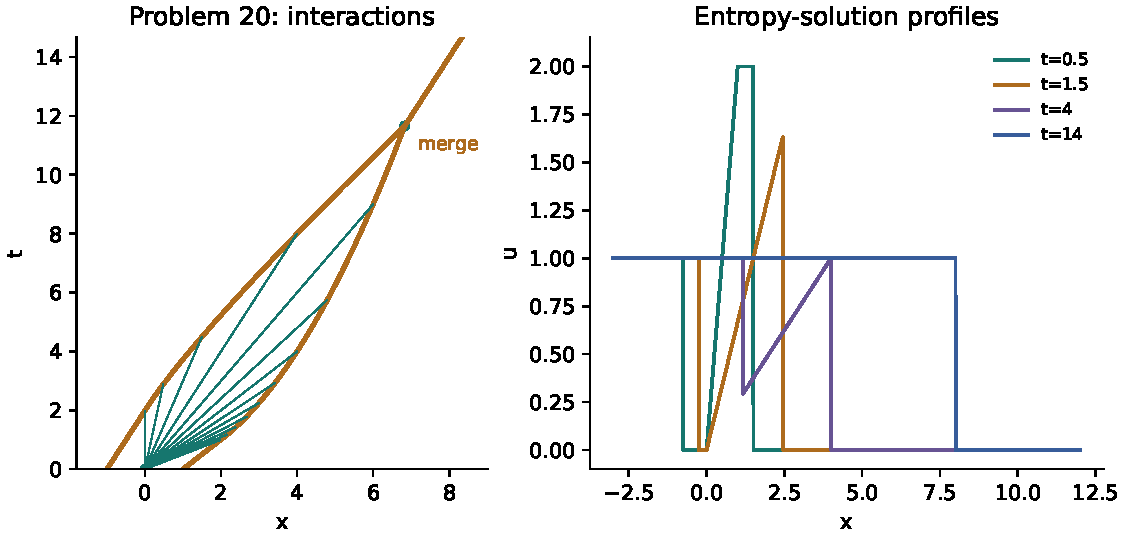
\includegraphics[width=\linewidth]{output/figures/ch03-interacting-waves.pdf}
\end{center}
\noindent\textit{Editorial figure.}
The space-time plot records interactions at $t=1$, $t=2$ and $T$;
the profiles show all four stages. Independent piecewise Hopf--Lax
minimization checks the formulas numerically away from shock ties.

% Evans second edition, section 3.6.
% English source: printed p. 158; PDF page 175 (1-based).
% Chinese section starts: checked against the chapter-opening list, PDF p. 79.
% Status: editorial study draft with detailed proofs and mathematical notes; no independent review.
\Needspace{65mm}
\section{References}
\label{sec:3-6}

The primary source is Lawrence C. Evans, \emph{Partial Differential
Equations}, second edition, Chapter 3, printed pp.~89--158
(local PDF pp.~106--175). The section order and explicit source
theorem identifiers follow that edition. The prose, expanded arguments,
Chinese notes, plots and exercise solutions are editorial reconstructions.

Evans's \S3.6 points to Courant--Hilbert for complete integrals;
Carath\'eodory, Garabedian, John, Chester and Sneddon for characteristics;
Lions, Rund and Benton for Hamilton--Jacobi theory; and Lax, Smoller
and Whitham for conservation laws.
The source attributes the HJ uniqueness argument to Douglis, the
entropy uniqueness argument to Oleinik, and the long-time estimates
to DiPerna, \emph{Indiana University Mathematics Journal} 24 (1975),
pp.~1047--1071.
These are source attributions and reading directions, not claims of
independent consultation of each listed work.

The Chinese chapter opening (PDF p.~79) lists section starts at printed
pp.~61, 64, 76, 90, 107, and 110 for \S3.1--\S3.6.
Selected Chinese pages for the local characteristic construction,
Hopf--Lax and shocks were checked as recorded in the chapter log.
A line-by-line comparison of the whole Chinese chapter has not been made.

\paragraph{Review boundary.}
The chapter invokes ODE existence and smooth dependence, implicit and
inverse function theorems, supporting hyperplanes for convex functions,
integration and weak calculus, Rademacher, and Gronwall as prerequisites.
The local existence proof includes the contact-compatibility step;
the two uniqueness arguments explicitly retain their different
selection classes. Long-time estimates are stated under convenient
sufficient convexity hypotheses, not optimal assumptions.
All 20 source exercises have solutions or exact pointers to full earlier
arguments. Numerical agreement with selected models and successful
compilation do not establish independent mathematical review.

